\hypertarget{scalability}{%
\section{Scalability}\label{scalability}}

\hypertarget{theoretical-speedups}{%
\subsection{Theoretical Speedups}\label{theoretical-speedups}}

\hypertarget{amdahl}{%
\subsubsection{Amdahl}\label{amdahl}}

Wie verkleiner sich die Laufzeit, wenn wir mehrere Prozessoren
einsetzen? Die Realität funktioniert nicht so wie die Theorie und es
lässt sich nicht alles parallelisieren.

\begin{figure}[H]
\centering
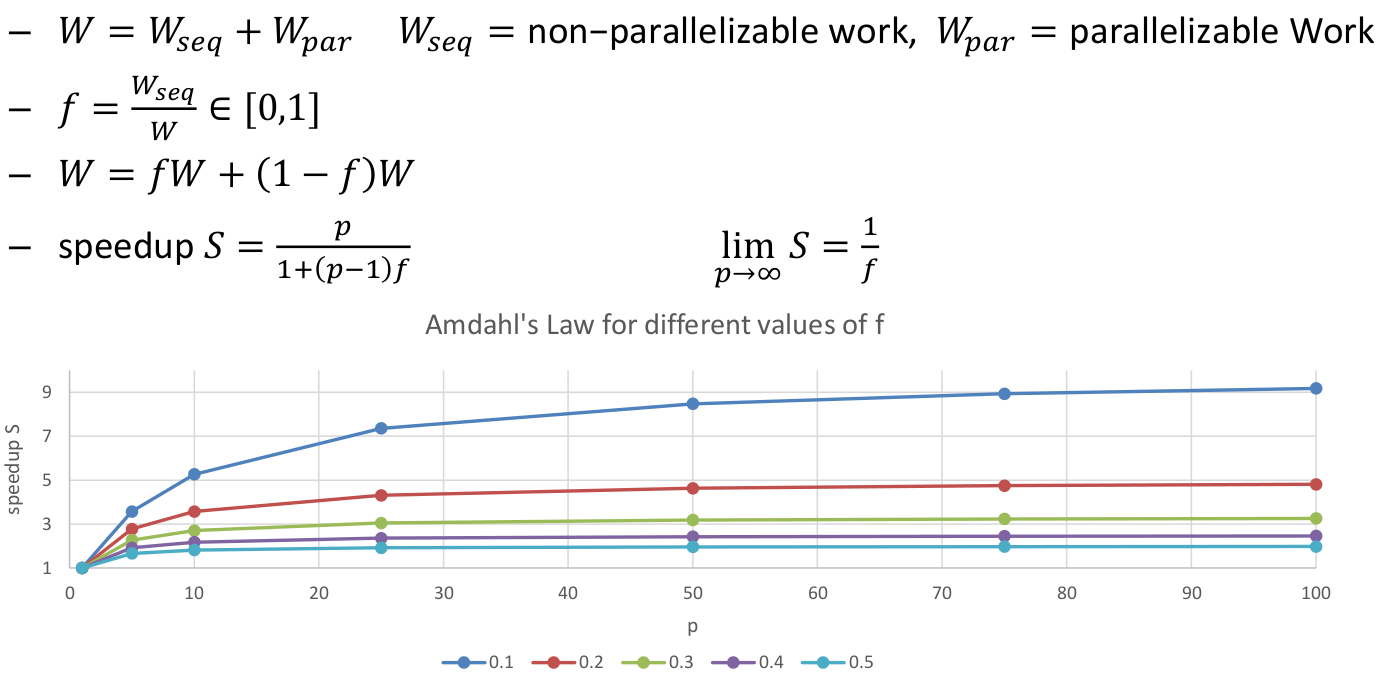
\includegraphics[width=0.6\textwidth]{figures/amdahl.png}
\caption{Amdahl}
\end{figure}

\textit{Mehr Notizen schriftlich in SW6.}

\hypertarget{gustafson-barsis}{%
\subsubsection{Gustafson-Barsis}\label{gustafson-barsis}}

Wie können wir die Laufzeit konstant halten wenn wir die Anzahl
Prozessoren und die Arbeitsmenge erhöhen?

\begin{figure}[H]
\centering
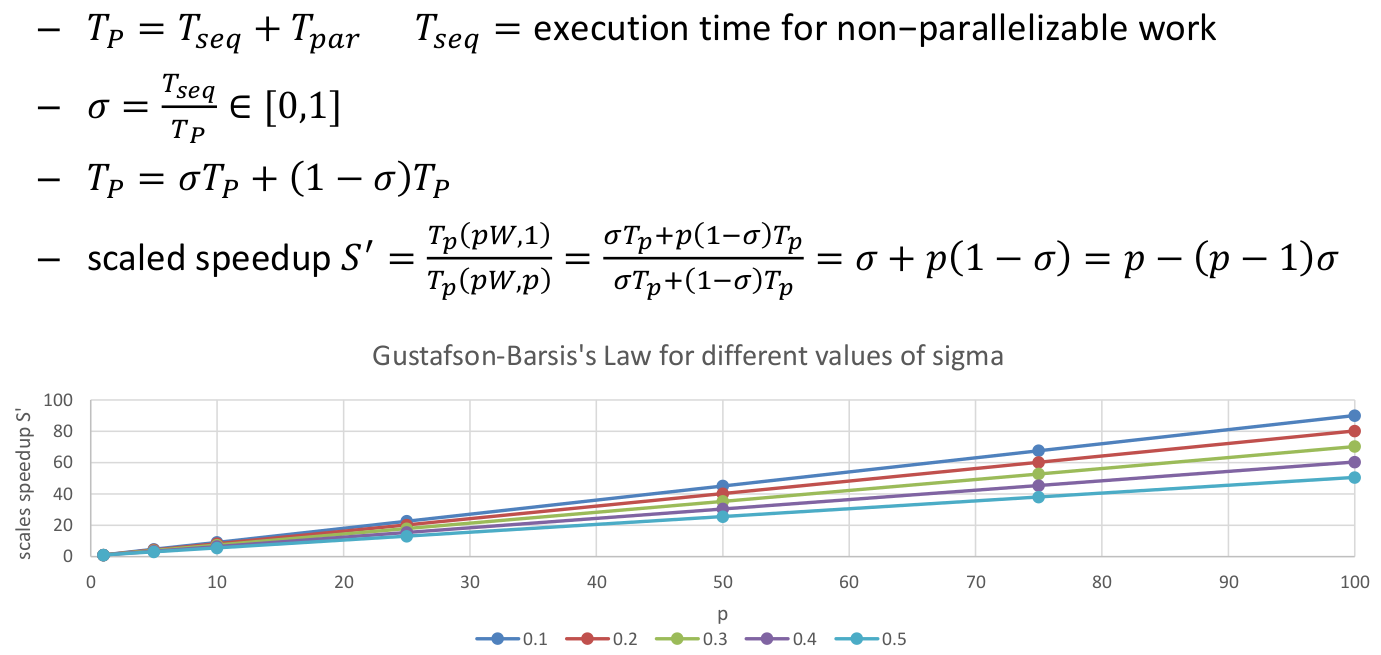
\includegraphics[width=0.7\textwidth]{figures/Gustafson-Barsis.png}
\caption{Gustafson-Barsis}
\end{figure}

\begin{figure}[H]
\centering
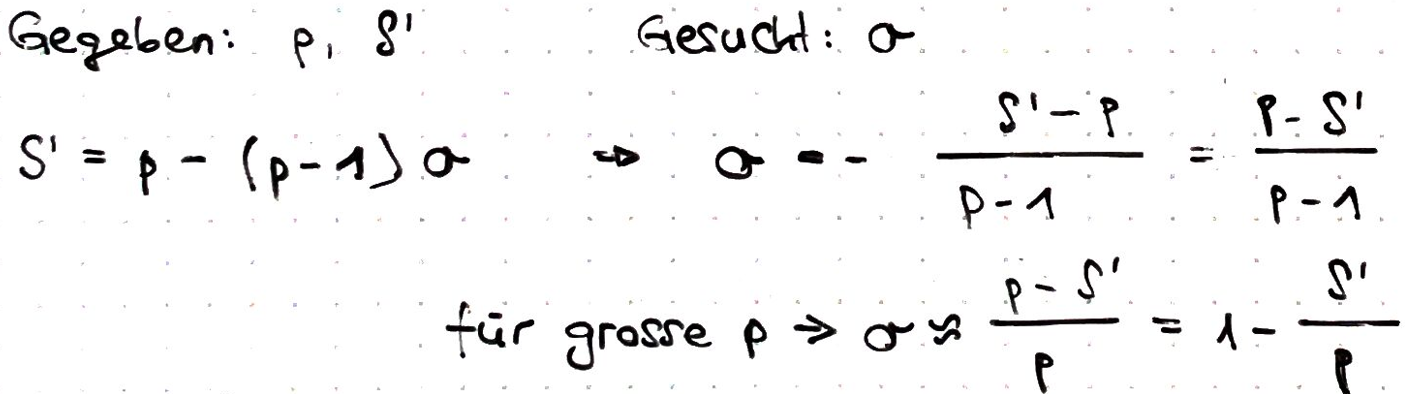
\includegraphics[width=0.5\textwidth]{figures/Gustafson-Barsis-Formeln.png}
\caption{Gustafson-Barsis Formeln}
\end{figure}

\hypertarget{karp-flatt}{%
\subsubsection{Karp-Flatt}\label{karp-flatt}}

Die Modelle von Amdahl und Gustafson-Barsis sind im Gegensatz zu
Karp-Flatt simpel. Karp-Flatt berücksichtigt zu den anderen Modellen
noch der Overhead, welcher von jedem einzelnen Prozessor generiert wird.

\begin{figure}[H]
\centering
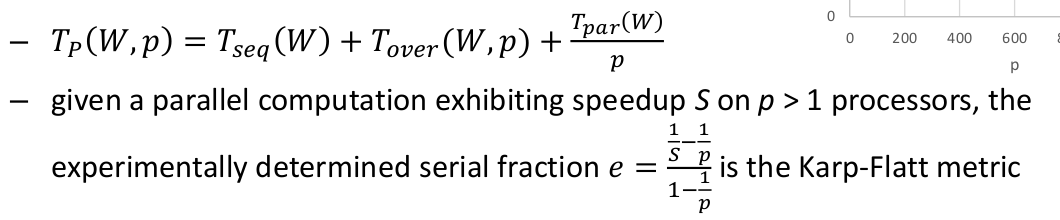
\includegraphics[width=0.7\textwidth]{figures/karp-flatt.png}
\caption{Karp-Flatt}
\end{figure}

\hypertarget{scalability-of-parallel-systems}{%
\subsection{Scalability of Parallel
Systems}\label{scalability-of-parallel-systems}}

\begin{figure}[H]
\centering
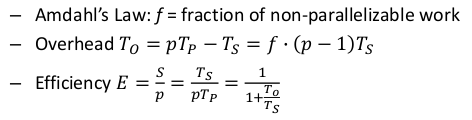
\includegraphics[width=0.7\textwidth]{figures/scalability-efficiency.png}
\caption{Overhead and Efficiency}
\end{figure}

How does the overhead $T_o$ and the efficiency $E$ change for a fixed
problem size?

\begin{itemize}
\tightlist
\item
  the value of $T_s$ remains constant
\item
  $T_o$ increases as a consequence of Amdahl's law
\item
  the overall efficiency of the parallel program goes down
\end{itemize}

\begin{figure}[H]
\centering
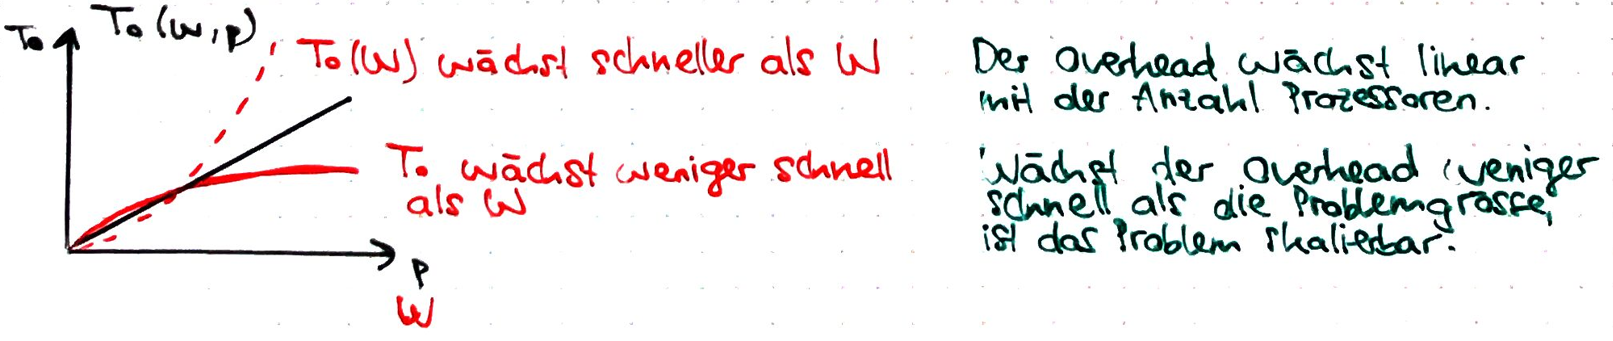
\includegraphics[width=0.7\textwidth]{figures/overhead.png}
\caption{Overhead}
\end{figure}

\begin{itemize}
\tightlist
\item
  in many cases, $T_o$ grows sub-linearly with respect to $W$
\item
  in such cases, the efficiency increases if the problem size is
  increased keeping the number of processing elements constant
\item
  for such systems, we can simultaneously increase the problem size and
  the number of processors to keep efficiency constant
\item
  $\Rightarrow$ such systems are called scalable parallel systems
\end{itemize}

Recall:

\begin{itemize}
\tightlist
\item
  $W$ is the asymptotic number of operations associated with the best
  serial algorithm to solve the problem: $W = \mathcal{O}(T_s)$
\item
  overhead $T_o (W, p)$ is a function of both problem size $W$ and the
  number of processing elements $p$
\item
  cost-optimal parallel systems have an efficiency of $\mathcal{O}(1)$
\end{itemize}

\begin{tcolorbox}[colback=red!5!white,colframe=red!75!black]
a scalable parallel system can always be made cost-optimal if the number of processing elements and the size of the computation are chosen appropriately. 
\end{tcolorbox}

\hypertarget{efficiency-as-function-of-p-and-w}{%
\subsubsection{Efficiency as Function of p and
W}\label{efficiency-as-function-of-p-and-w}}

\begin{itemize}
\tightlist
\item
  Fixe Problem Grösse $W$

  \begin{itemize}
  \tightlist
  \item
    Wenn wir die Problemgrösse $W$ belassen und nur die Anzahl Prozessoren
    erhöhen, nimmt der Overhead zu und somit die Effizienz ab.
  \item
    Dies gilt für alle Systeme
  \end{itemize}
\item
  Fixe Anzahl Prozessoren

  \begin{itemize}
  \tightlist
  \item
    Wenn wir die Anzahl Prozessoren belassen und nur die Problemgrösse
    erhöhen, nimmt die Effizienz zu.
  \item
    Dies gilt nur für skalierbare Systeme
  \end{itemize}
\item
  Kosten-Optimiertes System

  \begin{itemize}
  \tightlist
  \item
    Wenn wir die Anzahl Prozessoren erhöhen müssen wir gleichzeitig
    irgendwie die Effizienz wieder erhöhen, damit wir die Effizienz bei
    1 behalten.
  \item
    Um die Effizienz zu erhöhen, lassen wir zusätzlich die Problemgrösse
    grösser werden.
  \item
    Die Effizienz kann so mit höherer Anzahl Prozessoren und grösserem
    Problem immer auf 1 behalten werden.
  \item
    Dies gilt nur für skalierbare Systeme.
  \end{itemize}
\end{itemize}

\hypertarget{isoefficiency-metric-of-scalability}{%
\subsection{Isoefficiency Metric of
Scalability}\label{isoefficiency-metric-of-scalability}}

\textbf{Keeping the efficiency fixed}: Wie muss sich $P$ zu $W$ verhalten,
damit wir die Effizienz beibehalten können? Diese Rate bewertet die
Skalierbarkeit des Systems: \textbf{The slower this rate, the better.} \\

We are searching for the Isoefficiency Metric: $W$ as a function $f(p)$ for
a fixed efficiency E. Goal: express $W$ as a function of p: \textbf{$W =
f(p)$}

\hypertarget{formel}{%
\subsubsection{Formel}\label{formel}}

\begin{itemize}
\tightlist
\item
  $W = \frac{E}{1-E} * T_o(W,p)$
\item
  Konstante $K = \frac{E}{1-E}$
\item
  Final: If the number of processing elements is increased from $p$ to $p'$,
  the problem size $W = n$ must be increased by a factor of $\frac{p' log p'}{p
  log p}$ to get the same efficiency as on $p$ processing elements.
\end{itemize}

\begin{tcolorbox}[colback=red!5!white,colframe=red!75!black]
$f(p) = \mathcal{O}(p * log(p))$
\end{tcolorbox}

\hypertarget{example}{%
\subsubsection{Example}\label{example}}

\begin{figure}[H]
\centering
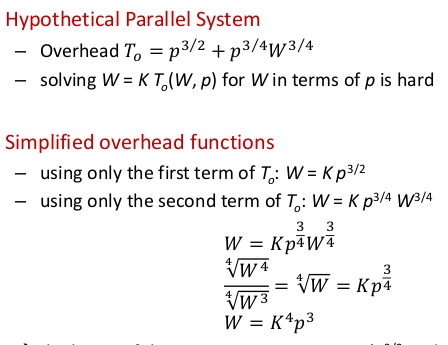
\includegraphics[width=0.5\textwidth]{figures/isoefficiency_example.png}
\caption{Isoefficiency Metric}
\end{figure}

\begin{itemize}
\tightlist
\item
  Das Beispiel zeigt ein komplizierteres Beispiel für die Formel des
  Overheads
\item
  Um die Isoeffizienz zu berechnen, wird der Term auseinandergenommen
  und diese einzeln berechnet
\item
  Am Schluss nimmt man die grösste der berechneten Isoeffizienz und
  verwirft die anderen
\end{itemize}

\hypertarget{cost-optimality-and-isoefficiency}{%
\subsubsection{Cost-Optimality and
Isoefficiency}\label{cost-optimality-and-isoefficiency}}

\begin{figure}[H]
\centering
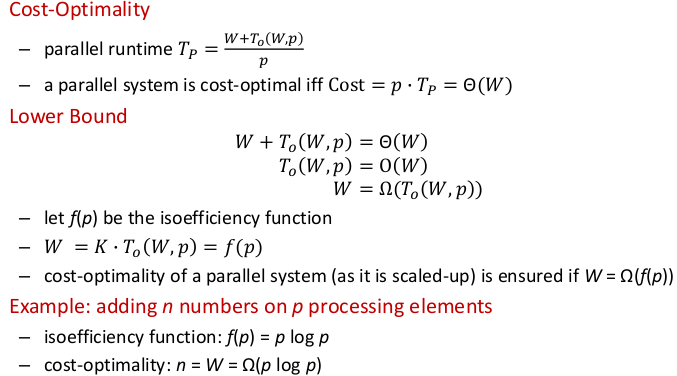
\includegraphics[width=0.7\textwidth]{figures/isoefficiency_costoptimality.png}
\caption{Cost-Optimality and Isoefficiency}
\end{figure}

\begin{itemize}
\tightlist
\item
  Ein paralleles system ist kostenoptimiertn, wenn die Effizienz
  konstant ist.
\item
  Das System ist kostenoptimiert, wenn W gleich schnell ansteigt wie
  f(p).
\item
  Die Konstante K kann dabei weggelassen werden.
\end{itemize}

\hypertarget{degree-of-concurrency}{%
\subsection{Degree of Concurrency}\label{degree-of-concurrency}}

\begin{itemize}
\tightlist
\item
  Definition: the maximum number of operations (tasks) that can be
  executed simultaneously at any time in a parallel algorithm

  \begin{itemize}
  \tightlist
  \item
    e.g.~in einem System das zu einem Zeitpunkt 8 Cores zur Verfügung
    hat, wäre dies 8. Egal ob es dann für andere Operationen nur noch
    einen Core zur Verfügung hat.
  \end{itemize}
\item
  it is independent of the parallel architecture
\item
  no more than $C(W)$ processing elements can be employed effectively
\end{itemize}

\hypertarget{effect-of-cw-on-isoefficiency}{%
\subsubsection{Effect of C(W) on
Isoefficiency}\label{effect-of-cw-on-isoefficiency}}

\begin{itemize}
\tightlist
\item
  isoefficiency due to concurrency is optimal only if $C(W) = \mathcal{O}(W)$
\item
  if $C(W) < \mathcal{O}(W)$ then the isoefficiency due to concurrency is
  worse than $\mathcal{O}(p)$

  \begin{itemize}
  \tightlist
  \item
    the overall isoefficiency function is given by the maximum of the
    isoefficiency functions due to concurrency, communication, and other
    overheads
  \end{itemize}
\end{itemize}

\hypertarget{minimum-execution-times}{%
\subsubsection{Minimum Execution Times}\label{minimum-execution-times}}

\begin{figure}[H]
\centering
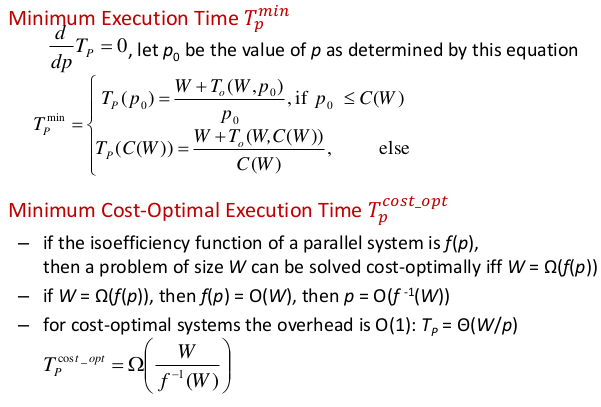
\includegraphics[width=0.7\textwidth]{figures/minimum-execution-time.png}
\caption{Minimum Execution Times}
\end{figure}

\clearpage
